%package list
\documentclass{article}
\usepackage[top=3cm, bottom=3cm, outer=3cm, inner=3cm]{geometry}
\usepackage{multicol}
\usepackage{graphicx}
\usepackage{url}
%\usepackage{cite}
\usepackage{hyperref}
\usepackage{array}
%\usepackage{multicol}
\newcolumntype{x}[1]{>{\centering\arraybackslash\hspace{0pt}}p{#1}}
\usepackage{natbib}
\usepackage{pdfpages}
\usepackage{multirow}
\usepackage[normalem]{ulem}
\useunder{\uline}{\ul}{}
\usepackage{svg}
\usepackage{xcolor}
\usepackage{listings}
\lstdefinestyle{ascii-tree}{
    literate={├}{|}1 {─}{--}1 {└}{+}1 
  }
\lstset{basicstyle=\ttfamily,
  showstringspaces=false,
  commentstyle=\color{red},
  keywordstyle=\color{blue}
}
%\usepackage{booktabs}
\usepackage{caption}
\usepackage{subcaption}
\usepackage{float}
\usepackage{array}

\newcolumntype{M}[1]{>{\centering\arraybackslash}m{#1}}
\newcolumntype{N}{@{}m{0pt}@{}}


%%%%%%%%%%%%%%%%%%%%%%%%%%%%%%%%%%%%%%%%%%%%%%%%%%%%%%%%%%%%%%%%%%%%%%%%%%%%
%%%%%%%%%%%%%%%%%%%%%%%%%%%%%%%%%%%%%%%%%%%%%%%%%%%%%%%%%%%%%%%%%%%%%%%%%%%%
\newcommand{\itemEmail}{schirinosne@unsa.edu.pe}
\newcommand{\itemStudent}{Sebastian Arley Chirinos Negrón}
\newcommand{\itemCourse}{Estructura de datos y Algoritmos}
\newcommand{\itemCourseCode}{1702124}
\newcommand{\itemSemester}{I}
\newcommand{\itemUniversity}{Universidad Nacional de San Agustín de Arequipa}
\newcommand{\itemFaculty}{Facultad de Ingeniería de Producción y Servicios}
\newcommand{\itemDepartment}{Departamento Académico de Ingeniería de Sistemas e Informática}
\newcommand{\itemSchool}{Escuela Profesional de Ingeniería de Sistemas}
\newcommand{\itemAcademic}{2023 - A}
\newcommand{\itemInput}{Del 29 Mayo 2023}
\newcommand{\itemOutput}{Al 05 Junio 2023}
\newcommand{\itemPracticeNumber}{02}
\newcommand{\itemTheme}{Revisión de elementos de programación}
%%%%%%%%%%%%%%%%%%%%%%%%%%%%%%%%%%%%%%%%%%%%%%%%%%%%%%%%%%%%%%%%%%%%%%%%%%%%
%%%%%%%%%%%%%%%%%%%%%%%%%%%%%%%%%%%%%%%%%%%%%%%%%%%%%%%%%%%%%%%%%%%%%%%%%%%%

\usepackage[english,spanish]{babel}
\usepackage[utf8]{inputenc}
\AtBeginDocument{\selectlanguage{spanish}}
\renewcommand{\figurename}{Figura}
\renewcommand{\refname}{Referencias}
\renewcommand{\tablename}{Tabla} %esto no funciona cuando se usa babel
\AtBeginDocument{%
	\renewcommand\tablename{Tabla}
}

\usepackage{fancyhdr}
\pagestyle{fancy}
\fancyhf{}
\setlength{\headheight}{30pt}
\renewcommand{\headrulewidth}{1pt}
\renewcommand{\footrulewidth}{1pt}
\fancyhead[L]{\raisebox{-0.2\height}{
\includegraphics[width=3cm]{img/logo_episunsa.png}}}
\fancyhead[C]{\fontsize{7}{7}\selectfont	\itemUniversity \\ \itemFaculty \\ \itemDepartment \\ \itemSchool \\ \textbf{\itemCourse}}
\fancyhead[R]{\raisebox{-0.2\height}{
\includegraphics[width=1.2cm]{img/logo_abet}}}
\fancyfoot[L]{Sebastian Chirinos Negrón}
\fancyfoot[C]{\itemCourse}
\fancyfoot[R]{Página \thepage}

% para el codigo fuente
\usepackage{listings}
\usepackage{color, colortbl}
\definecolor{dkgreen}{rgb}{0,0.6,0}
\definecolor{gray}{rgb}{0.5,0.5,0.5}
\definecolor{mauve}{rgb}{0.58,0,0.82}
\definecolor{codebackground}{rgb}{72, 0.95, 0.92}
\definecolor{tablebackground}{rgb}{0.8, 0, 0}

\lstset{frame=tb,
	language=bash,
	aboveskip=3mm,
	belowskip=3mm,
	showstringspaces=false,
	columns=flexible,
	basicstyle={\small\ttfamily},
	numbers=none,
	numberstyle=\tiny\color{gray},
	keywordstyle=\color{blue},
	commentstyle=\color{dkgreen},
	stringstyle=\color{mauve},
	breaklines=true,
	breakatwhitespace=true,
	tabsize=3,
	backgroundcolor= \color{codebackground},
}

\begin{document}
	
	\vspace*{10px}
	
	\begin{center}	
		\fontsize{17}{17} \textbf{ Informe de Laboratorio \itemPracticeNumber}
	\end{center}
	\centerline{\textbf{\Large Tema: \itemTheme}}
	%\vspace*{0.5cm}	

	\begin{flushright}
		\begin{tabular}{|M{2.5cm}|N|}
			\hline 
			\rowcolor{tablebackground}
			\color{white} \textbf{Nota}  \\
			\hline 
			     \\[30pt]
			\hline 			
		\end{tabular}
	\end{flushright}	

	\begin{table}[H]
		\begin{tabular}{|x{4.7cm}|x{4.8cm}|x{4.8cm}|}
			\hline 
			\rowcolor{tablebackground}
			\color{white} \textbf{Estudiante} & \color{white}\textbf{Escuela}  & \color{white}\textbf{Asignatura}   \\
			\hline 
			{\itemStudent \par \itemEmail} & \itemSchool & {\itemCourse \par Semestre: \itemSemester \par Código: \itemCourseCode}     \\
			\hline 			
		\end{tabular}
	\end{table}		
	
	\begin{table}[H]
		\begin{tabular}{|x{4.7cm}|x{4.8cm}|x{4.8cm}|}
			\hline 
			\rowcolor{tablebackground}
			\color{white}\textbf{Laboratorio} & \color{white}\textbf{Tema}  & \color{white}\textbf{Duración}   \\
			\hline 
			\itemPracticeNumber & \itemTheme & 04 horas   \\
			\hline 
		\end{tabular}
	\end{table}
	
	\begin{table}[H]
		\begin{tabular}{|x{4.7cm}|x{4.8cm}|x{4.8cm}|}
			\hline 
			\rowcolor{tablebackground}
			\color{white}\textbf{Semestre académico} & \color{white}\textbf{Fecha de inicio}  & \color{white}\textbf{Fecha de entrega}   \\
			\hline 
			\itemAcademic & \itemInput &  \itemOutput  \\
			\hline 
		\end{tabular}
	\end{table}
	
	\section{Tarea}
	\begin{itemize}		
		\item Invertir un matriz de enteros (2 pts)
		\item Rotación a la Izquierda (3 pts)
		\item Triángulo recursivo (4 pts)
		
	\end{itemize}
		
	\section{Equipos, materiales y temas utilizados}
	\begin{itemize}
		\item Realizar ejercicios en temas de Estructuras de datos, tipos de datos abstractos, bucles, Arrays, Listas enlazadas, Recursión
		\item Java
		\item TAD
		\item Arrays
		\item C.m. Construye responsablemente soluciones haciendo uso de estructuras de datos y algoritmos, siguiendo un proceso adecuado para resolver problemas computacionales que se ajustan al uso de los recursos disponibles y a especificaciones concretas.
		
	\end{itemize}
	
	\section{URL de Repositorio Github}
	\begin{itemize}
		\item URL del Repositorio GitHub para clonar o recuperar.
		\item \url{https://github.com/BastleyNait/EDA-LAB-B-23A.git}
		\item URL para el laboratorio 04 en el Repositorio GitHub.
		\item \url{https://github.com/BastleyNait/EDA-LAB-B-23A/tree/main/lab02}
	\end{itemize}
	
	\section{Ejercicios designados}

	\subsection{Ejercicio 1}
	\begin{itemize}	
		\item El programa crea un array, invierte sus elementos y luego los imprime en la consola.
	\end{itemize}	
	
	\lstinputlisting[language=Java, caption={Ejercicio01.java},numbers=left,]{src/Ejercicio01.java}	

	\begin{itemize}	
		\item Crea un array llamado A con elementos 1, 2 y 3.
		\item Llama al método invertirArray pasando el array A como argumento y almacena el resultado en un nuevo array llamado B.
		\item Llama al método imprimir pasando el array invertido B como argumento.
		\item El método invertirArray recibe un array A como argumento, crea un nuevo array llamado Ain con la misma longitud que A y realiza un bucle para invertir los elementos de A en Ain, asignando el elemento en la posición i de A al elemento en la posición j de Ain.
		\item El método imprimir recibe un array a como argumento y realiza un bucle para imprimir cada elemento del array separado por un espacio. Luego imprime una nueva línea.
	\end{itemize}

	\begin{itemize}	
		\item Ejecucion del codigo:
	\end{itemize}	
	
	\begin{figure}[H]
		\centering
		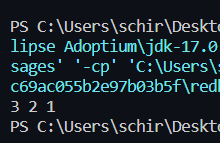
\includegraphics[width=0.7\textwidth,keepaspectratio]{img/Ejercicio01.png}
		%\includesvg{img/automata.svg}
		%\label{img:mot2}
		%\caption{Product backlog.}
	\end{figure}

	%%%%%%%%%%%%%%%%%%%%%%%%%%%%%%%%%%%%%%%%%%%%%%%%%%%%%%%%%%%%%%%%%%%%%%%%%%%%%%%%%%%%%%%%%%%%%
	\subsection{Ejercicio 2}
	\begin{itemize}	
		\item el programa crea un array, realiza una rotación hacia la izquierda de los elementos del array y luego los imprime en la consola.
	\end{itemize}	
	
	\lstinputlisting[language=Java, caption={Ejercicio02.java},numbers=left,]{src/Ejercicio02.java}	

	\begin{itemize}	
		\item Crea un array llamado A con elementos 1, 2, 3, 4 y 5.
		\item Llama al método rotarIzquierdaArray pasando el array A y el valor 2 como argumentos, y almacena el resultado en un nuevo array llamado B.
		\item Llama al método imprimir pasando el array rotado B como argumento.
		\item El método rotarIzquierdaArray recibe un array A y un valor d como argumentos, crea un nuevo array llamado Aiz con la misma longitud que A, y realiza un bucle para rotar los elementos de A hacia la izquierda. Calcula la nueva posición j para el elemento en la posición i después de la rotación y asigna el elemento correspondiente de A al elemento en la posición j de Aiz.
		\item El método imprimir recibe un array a como argumento y realiza un bucle para imprimir cada elemento del array separado por un espacio. Luego imprime una nueva línea.
	\end{itemize}

	\begin{itemize}	
		\item Ejecucion del codigo:
	\end{itemize}	
	
	\begin{figure}[H]
		\centering
		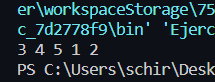
\includegraphics[width=0.7\textwidth,keepaspectratio]{img/Ejercicio02.png}
		%\includesvg{img/automata.svg}
		%\label{img:mot2}
		%\caption{Product backlog.}
	\end{figure}
%%%%%%%%%%%%%%%%%%%%%%%%%%%%%%%%%%%%%%%%%%%%%%%%%%%%%%%%%%%%%%%%%%%%%%%%%%%%%%%%%%%%%%%%%%%%%%%%%%%%%%%%%%
%%%%%%%%%%%%%%%%%%%%%%%%%%%%%%%%%%%%%%%%%%%%%%%%%%%%%%%%%%%%%%%%%%%%%%%%%%%%%%%%%%%%%%%%%%%%%
\subsection{Ejercicio 3}
\begin{itemize}	
	\item El programa utiliza la recursión para imprimir un triángulo de asteriscos con la cantidad de filas especificada.
\end{itemize}	

\lstinputlisting[language=Java, caption={Ejercicio03.java},numbers=left,]{src/Ejercicio03.java}	

\begin{itemize}	
	\item El método trianguloRecursivo recibe un parámetro base que representa la cantidad de filas del triángulo. Si la base llega a ser 0, la recursión se detiene y no hay nada más que imprimir. En caso contrario, se realiza lo siguiente:
	\item Se realiza un bucle para imprimir asteriscos en cada nivel del triángulo. La cantidad de asteriscos en cada nivel está determinada por la variable contador.
	\item Después de imprimir los asteriscos del nivel actual, se imprime una nueva línea.
	\item Se incrementa el valor de contador para el siguiente nivel del triángulo.
	\item Se realiza una llamada recursiva al método trianguloRecursivo, disminuyendo la base en 1 en cada llamada.
	\item La recursión se repite hasta que la base llegue a ser 0 y se complete la impresión del triángulo de asteriscos.
\end{itemize}
\clearpage

\begin{itemize}	
	\item Ejecucion del codigo:
\end{itemize}	

\begin{figure}[H]
	\centering
	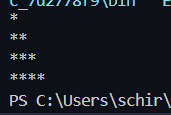
\includegraphics[width=0.7\textwidth,keepaspectratio]{img/Ejercicio03.png}
	%\includesvg{img/automata.svg}
	%\label{img:mot2}
	%\caption{Product backlog.}
\end{figure}
%%%%%%%%%%%%%%%%%%%%%%%%%%%%%%%%%%%%%%%%%%%%%%%%%%%%%%%%%%%%%%%%%%%%%%%%%%%%%%%%%%%%%%%%%%%%%%%%%%%%%%%%%%

	\subsection{Commits del trabajo}
	\begin{itemize}	
		\item Acá estan algunos de los commits mas importantes en este trabajo:
	\end{itemize}	
	
	\begin{figure}[H]
		\centering
		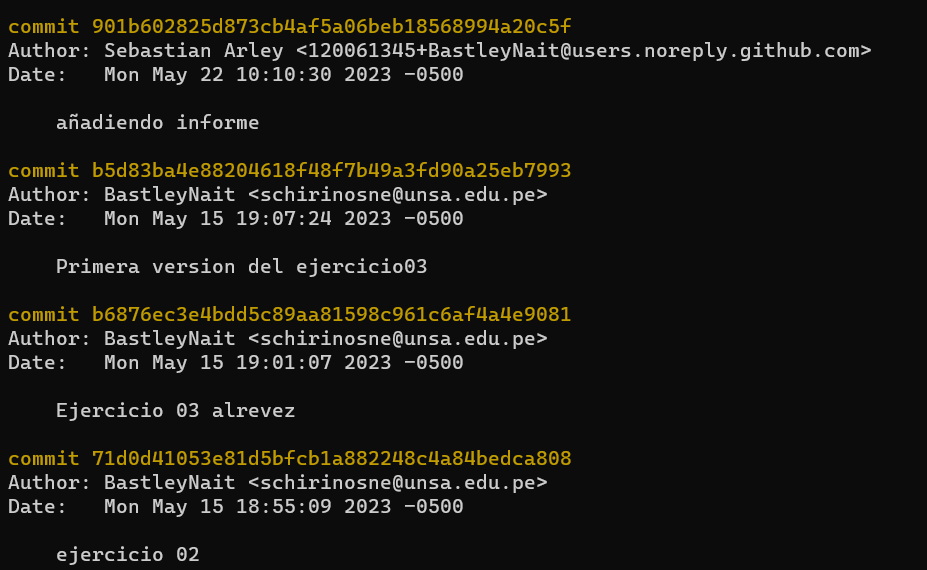
\includegraphics[width=0.7\textwidth,keepaspectratio]{img/Commits.png}
		%\includesvg{img/automata.svg}
		%\label{img:mot2}
		%\caption{Product backlog.}
	\end{figure}


%%%%%%%%%%%%%%%%%%%%%%%%%%%%%%%%%%%%%%%%%%%%%%%%%%%%%%%%%%%%%%%%%%%%%%%%%%%%%%%%%%
	
		
	\subsection{Estructura de laboratorio 01}
	\begin{itemize}	
		\item El contenido que se entrega en este laboratorio es el siguiente:
	\end{itemize}
	
\begin{lstlisting}[style=ascii-tree]
lab02/
|   Ejercicio01.java
|   Ejercicio02.java
|   Ejercicio03.java
|   lab02.iml
|
\---latex
    |   EDA_lab02_schirinosne.pdf
    |   EDA_lab02_schirinosne.tex
    |
    +---img
    |       Commits.png
    |       Ejercicio01.png
    |       Ejercicio02.png
    |       Ejercicio03.png
    |       logo_abet.png
    |       logo_episunsa.png
    |       logo_unsa.jpg
    |
    \---src
            Ejercicio01.java
            Ejercicio02.java
            Ejercicio03.java
\end{lstlisting}    

\section{Pregunta: ¿Qué diferencia hay entre un List y un ArrayList en Java?
}
	\begin{itemize}
		\item La diferencia entre un List y un ArrayList en Java se encuentra en la implementación y en las características específicas de cada una:
		\item List es una interfaz en Java que define el comportamiento general de una lista, incluyendo operaciones como agregar elementos, acceder a elementos por índice, eliminar elementos y otras funcionalidades comunes. Es una interfaz de alto nivel que no especifica la implementación subyacente.
		\item ArrayList, por otro lado, es una implementación específica de la interfaz List. Representa una lista basada en un array dinámico, lo que significa que internamente utiliza un array para almacenar los elementos y se redimensiona automáticamente según sea necesario. Proporciona un acceso rápido a los elementos por índice y es eficiente para operaciones de lectura y escritura. Sin embargo, la inserción o eliminación de elementos en posiciones intermedias puede ser costosa en términos de rendimiento, ya que puede requerir desplazar los elementos.
		
	\end{itemize}	
\section{Pregunta: ¿Qué beneficios y oportunidades ofrecen las clases genéricas en Java?}
	\begin{itemize}
		\item En cuanto a las clases genéricas en Java, ofrecen beneficios y oportunidades significativas:
		\item Permiten la creación de clases y métodos que pueden ser parametrizados con tipos específicos. Esto proporciona un alto grado de reutilización de código, ya que una clase o método genérico puede ser utilizado con diferentes tipos de datos sin necesidad de escribir implementaciones específicas para cada tipo.
		\item Ayudan a garantizar la seguridad de tipos en tiempo de compilación. Al especificar el tipo de datos que se utilizará en una clase genérica, el compilador de Java puede detectar posibles errores de tipos antes de la ejecución del programa, lo que ayuda a evitar errores comunes y a mejorar la robustez del código.
		\item Mejoran la legibilidad y mantenibilidad del código. Al utilizar clases genéricas, se puede expresar de manera más clara y concisa la intención y el propósito del código. Además, al utilizar tipos genéricos, se evita la necesidad de conversiones explícitas entre tipos en muchas situaciones.
		\item Permiten la creación de estructuras de datos genéricas y algoritmos reutilizables. Las clases genéricas son especialmente útiles para implementar estructuras de datos como listas, pilas, colas, árboles, etc., que pueden manejar diferentes tipos de datos de manera flexible y segura.
	\end{itemize}		

\section{Referencias}
\begin{itemize}			
	\item \url{https://www.w3schools.com/java/}
	\item \url{https://docs.oracle.com/javase/7/docs/api/java/util/List.html}
	\item \url{https://docs.oracle.com/javase/tutorial/java/generics/types.html}

\end{itemize}	

	
%\clearpage
%\bibliographystyle{apalike}
%\bibliographystyle{IEEEtranN}
%\bibliography{bibliography}
			
\end{document}